%
% chapter.tex
%
% (c) 2020 Prof Dr Andreas Müller, Hochschule Rapperswil
%
\chapter{Matrizengruppen
\label{buch:chapter:matrizengruppen}}
\lhead{Matrizengruppen}
\rhead{}
Matrizen können dazu verwendet werden, Symmetrien von geometrischen oder
physikalischen Systemen zu beschreiben.
Neben diskreten Symmetrien wie zum Beispiel Spiegelungen gehören dazu
auch kontinuierliche Symmetrien wie Translationen oder Invarianz einer
phyisikalischen Grösse über die Zeit.
Solche Symmetrien müssen durch Matrizen beschrieben werden können,
die auf stetige oder sogar differenzierbare Art von der Zeit abhängen.
Die Menge der Matrizen, die zur Beschreibung solcher Symmetrien benutzt
werden, muss also eine zusätzliche Struktur haben, die ermöglicht, 
sinnvoll über Stetigkeit und Differenzierbarkeit bei Matrizen
zu sprechen.

Die Menge der Matrizen bilden zunächst eine Gruppe,
die zusätzliche differenziarbare Struktur macht daraus
eine sogenannte Lie-Gruppe.
Die Ableitungen nach einem Parameter liegen in der sogenannten
Lie-Algebra, einer Matrizen-Algebra mit dem antisymmetrischen
Lie-Klammer-Produkt $[A,B]=AB-BA$, auch Kommutator genannt.
Lie-Gruppe und Lie-Algebra sind eng miteinander verknüpft,
so eng, dass sich die meisten Eigenschaften der Gruppe aus den Eigenschaften
der Lie-Gruppe aus der Lie-Algebra ableiten lassen.
Die Verbindung wird hergestellt durch die Exponentialabbildung.
Ziel dieses Kapitels ist, die Grundzüge dieses interessanten 
Zusammenhangs darzustellen.

%
% symmetrien.tex -- Symmetrien
%
% (c) 2021 Prof Dr Andreas Müller, OST Ostschweizer Fachhochschule
%
\bgroup
\definecolor{darkgreen}{rgb}{0,0.6,0}
\begin{frame}[t]
\setlength{\abovedisplayskip}{5pt}
\setlength{\belowdisplayskip}{5pt}
\frametitle{Symmetrien}
\vspace{-20pt}
\begin{columns}[t,onlytextwidth]
\begin{column}{0.48\textwidth}
\begin{block}{Diskrete Symmetrien}
\begin{itemize}
\item<2->
Ebenen-Spiegelung:
\[
{\tiny
\begin{pmatrix*}[r] x_1\\x_2\\x_3 \end{pmatrix*}
}
\mapsto
{\tiny
\begin{pmatrix*}[r]-x_1\\x_2\\x_3 \end{pmatrix*}
}
\uncover<4->{\!,\;
\vec{x}
\mapsto
\vec{x} -2 (\vec{n}\cdot\vec{x}) \vec{n}
}
\]
\vspace{-10pt}
\begin{center}
\begin{tikzpicture}[>=latex,thick]
\def\a{10}
\def\b{50}
\def\r{2}
\coordinate (O) at (0,0);
\coordinate (A) at (\b:\r);
\coordinate (B) at ({180+2*\a-\b}:\r);
\coordinate (C) at ({90+\a}:{\r*cos(90+\a-\b)});
\coordinate (N) at (\a:2);
\coordinate (D) at (\a:{\r*cos(\b-\a)});
\uncover<3->{
\clip (-2.5,-0.45) rectangle (2.5,1.95);

	\fill[color=darkgreen!20] (O) -- ({\a-90}:0.2) arc ({\a-90}:\a:0.2)
		-- cycle;
	\draw[->,color=darkgreen] (O) -- (N);
	\node[color=darkgreen] at (N) [above] {$\vec{n}$};


	\fill[color=blue!20] (C) -- ($(C)+(\a:0.2)$) arc (\a:{90+\a}:0.2)
		-- cycle;
	\fill[color=red] (O) circle[radius=0.06];
	\draw[color=red] ({\a-90}:2) -- ({\a+90}:2);
	\fill[color=blue] (C) circle[radius=0.06];
	\draw[color=blue,line width=0.1pt] (A) -- (D);
	\node[color=darkgreen] at (D) [below,rotate=\a]
		{$(\vec{n}\cdot\vec{x})\vec{n}$};
	\draw[color=blue,line width=0.5pt] (A)--(B);

	\node[color=blue] at (A) [above right] {$\vec{x}$};
	\node[color=blue] at (B) [above left] {$\vec{x}'$};

	\node[color=red] at (O) [below left] {$O$};

	\draw[->,color=blue,shorten <= 0.06cm,line width=1.4pt] (O) -- (A);
	\draw[->,color=blue,shorten <= 0.06cm,line width=1.4pt] (O) -- (B);
}

\end{tikzpicture}
\end{center}
\vspace{-5pt}
$\vec{n}$ ein Einheitsnormalenvektor auf der Ebene, $|\vec{n}|=1$
\item<5->
Punkt-Spiegelung:
\[
{\tiny
\begin{pmatrix*}[r] x_1\\x_2\\x_3 \end{pmatrix*}
}
\mapsto
-
{\tiny
\begin{pmatrix*}[r]x_1\\x_2\\x_3 \end{pmatrix*}
}
\]
\end{itemize}
\end{block}
\end{column}
\begin{column}{0.48\textwidth}
\uncover<6->{%
\begin{block}{Kontinuierliche Symmetrien}
\begin{itemize}
\item<7-> Translation:
\(
\vec{x} \mapsto \vec{x} + \vec{t}
\)
\item<8-> Drehung:
\vspace{-3pt}
\begin{center}
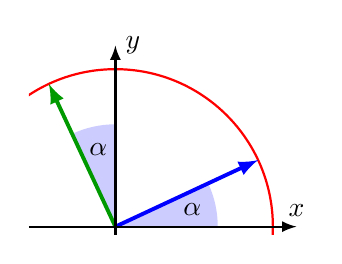
\begin{tikzpicture}[>=latex,thick]
\def\a{25}
\def\r{1.3}
\coordinate (O) at (0,0);
\begin{scope}
\clip (-1.1,-0.1) rectangle (2.3,2.3);
\draw[color=red] (O) circle[radius=2];
\fill[color=blue!20] (O) -- (0:\r) arc (0:\a:\r) -- cycle;
\fill[color=blue!20] (O) -- (90:\r) arc (90:{90+\a}:\r) -- cycle;
\node at ({0.5*\a}:1) {$\alpha$};
\node at ({90+0.5*\a}:1) {$\alpha$};
\draw[->,color=blue,line width=1.4pt] (O) -- (\a:2);
\draw[->,color=darkgreen,line width=1.4pt] (O) -- ({90+\a}:2);
\end{scope}
\draw[->] (-1.1,0) -- (2.3,0) coordinate[label={$x$}];
\draw[->] (0,-0.1) -- (0,2.3) coordinate[label={right:$y$}];
\end{tikzpicture}
\end{center}
\[
\uncover<9->{%
\begin{pmatrix}x\\y\end{pmatrix}
\mapsto
\begin{pmatrix}
{\color{blue}\cos\alpha}&{\color{darkgreen}-\sin\alpha}\\
{\color{blue}\sin\alpha}&{\color{darkgreen}\phantom{-}\cos\alpha}
\end{pmatrix}
\begin{pmatrix}x\\y\end{pmatrix}
}
\]
\end{itemize}
\end{block}}
\vspace{-10pt}
\uncover<10->{%
\begin{block}{Definition}
Längen/Winkel bleiben erhalten
\\
\uncover<11->{%
$\Rightarrow$ $\exists$ Erhaltungsgrösse}
\end{block}}
\end{column}
\end{columns}
\end{frame}
\egroup

%
% lie-gruppen.tex -- Lie-Gruppebn
%
% (c) 2020 Prof Dr Andreas Müller, Hochschule Rapperswil
%
\section{Lie-Gruppen
\label{buch:section:lie-gruppen}}
\rhead{Lie-Gruppen}

\subsection{Drehungen in der Ebene
\label{buch:gruppen:drehungen2d}}
Drehungen der Ebene können in einer orthonormierten Basis durch
Matrizen der Form
\[
D_{\alpha}
=
\begin{pmatrix}
\cos\alpha&-\sin\alpha\\
\sin\alpha& \cos\alpha
\end{pmatrix}
\]
dargestellt werden.
Wir bezeichnen die Menge der Drehmatrizen in der Ebene mit
$\operatorname{SO}(2)\subset\operatorname{GL}_2(\mathbb{R})$.
Die Abbildung
\[
D_{\bullet}
\colon
\mathbb{R}\to \operatorname{SO}(2)
:
\alpha \mapsto D_{\alpha}
\]
hat die Eigenschaften
\begin{align*}
D_{\alpha+\beta}&= D_{\alpha}D_{\beta}
\\
D_0&=I
\\
D_{2k\pi}&=I\qquad \forall k\in\mathbb{Z}.
\end{align*}
Daraus folgt zum Beispiel, dass $D_{\bullet}$ eine $2\pi$-periodische
Funktion ist.
$D_{\bullet}$ bildet die Menge der Winkel $[0,2\pi)$ bijektiv auf
die Menge der Drehmatrizen in der Ebene ab.

Ein alternatives Bild für die Drehungen der Ebene kann man in der komplexen
Ebene $\mathbb{C}$ erhalten.
Die Multiplikation mit der komplexen Zahl $e^{i\alpha}$ beschreibt eine
Drehung der komplexen Ebene um den Winkel $\alpha$.
Die Zahlen der Form $e^{i\alpha}$ haben den Betrag $1$ und die Abbildung
\[
f\colon \mathbb{R}\to \mathbb{C}:\alpha \mapsto e^{i\alpha}
\]
hat die Eigenschaften
\begin{align*}
f(\alpha+\beta) &= f(\alpha)f(\beta)
\\
f(0)&=1
\\
f(2\pi k)&=1\qquad\forall k\in\mathbb{Z},
\end{align*}
die zu den Eigenschaften der Abbildung $\alpha\mapsto D_{\alpha}$ 
analog sind.

Jede komplexe Zahl $z$ vom Betrag $1$ kann geschrieben werden in der Form
$z=e^{i\alpha}$, die Abbildung $f$ ist also eine Parametrisierung des
Einheitskreises in der Ebene.
Wir bezeichen $S^1=\{z\in\mathbb{C}\;|\; |z|=1\}$ die komplexen Zahlen vom
Betrag $1$.
$S^1$ ist eine Gruppe bezüglich der Multiplikation, da für jede Zahl
$z,w\in S^1$ gilt
$|z^{-1}|=1$ und $|zw|=1$ und damit $z^{-1}\in S^1$ und $zw\in S^1$.

Zu einer komplexen Zahl $z\in S^1$ gibt es einen bis auf Vielfache
von $2\pi$ eindeutigen Winkel $\alpha(z)$ derart, dass $e^{i\alpha(z)}=z$.
Damit kann man jetzt die Abbildung
\[
\varphi
\colon
S^1\to \operatorname{SO}(2)
:
z\mapsto  D_{\alpha(z)}
\]
konstruieren.
Da $D_{\alpha}$ $2\pi$-periodisch ist, geben um Vielfache
von $2\pi$ verschiedene Wahlen von $\alpha(z)$ die gleiche
Matrix $D_{\alpha(z)}$, die Abbildung $\varphi$ ist daher
wohldefiniert.
$\varphi$ erfüllt ausserdem die Bedingungen
\begin{align*}
\varphi(z_1z_2)
&=
D_{\alpha(z_1z_2)}
=
D_{\alpha(z_1)+\alpha(z_2)}
=
D_{\alpha(z_1)}D_{\alpha(z_2)}
=
\varphi(z_1)\varphi(z_2)
\\
\varphi(1)
&=
D_{\alpha(1)}
=
D_0
=
I
\end{align*}
Die Abbildung $\varphi$ ist ein Homomorphismus der Gruppe $S^1$
in die Gruppe $\operatorname{SO}(2)$.
Die Menge der Drehmatrizen in der Ebene kann also mit dem Einheitskreis
in der komplexen Ebene identifiziert werden.

\subsection{Isometrien von $\mathbb{R}^n$
\label{buch:gruppen:isometrien}}
Lineare Abbildungen der Ebene $\mathbb{R}^n$ mit dem üblichen Skalarprodukt
können durch $n\times n$-Matrizen beschrieben werden.
Die Matrizen, die das Skalarprodukt erhalten, bilden eine Gruppe,
die in diesem Abschnitt genauer untersucht werden soll.
Eine Matrix $A\in M_{2}(\mathbb{R})$ ändert das Skalarprodukt nicht, wenn
für jedes beliebige Paar $x,y$ von Vektoren gilt
$\langle Ax,Ay\rangle = \langle x,y\rangle$.
Das Standardskalarprodukt kann mit dem Matrixprodukt ausgedrückt werden:
\[
\langle Ax,Ay\rangle
=
(Ax)^tAy
=
x^tA^tAy
=
x^ty
=
\langle x,y\rangle
\]
für jedes Paar von Vektoren $x,y\in\mathbb{R}$.

Mit dem Skalarprodukt kann man auch die Matrixelemente einer Matrix
einer Abbildung $f$ in der Standardbasis bestimmen.
Das Skalarprodukt $\langle e_i, v\rangle$ ist die Länge der Projektion
des Vektors $v$ auf die Richtung $e_i$.
Die Komponenten von $Ae_j$ sind daher $a_{ij}=\langle e_i,f(e_j)\rangle$.
Die Matrix $A$ der Abbildung $f$ hat also die Matrixelemente
$a_{ij}=e_i^tAe_j$.


\subsection{Die Gruppe $\operatorname{SU}(2)$
\label{buch:gruppen:su2}}

%
% lie-algebren.tex -- Lie-Algebren
%
% (c) 2020 Prof Dr Andreas Müller, Hochschule Rapperswil
%
\section{Lie-Algebren
\label{buch:section:lie-algebren}}
\rhead{Lie-Algebren}
Im vorangegangenen Abschnitt wurde gezeigt, dass alle beschriebenen
Matrizengruppen als Untermannigfaltigkeiten im $n^2$-dimensionalen
Vektorraum $M_n(\mathbb{R}9$ betrachtet werden können.
Die Gruppen haben damit nicht nur die algebraische Struktur einer
Matrixgruppe, sie haben auch die geometrische Struktur einer 
Mannigfaltigkeit.
Insbesondere ist es sinnvoll, von Ableitungen zu sprechen.

Eindimensionale Untergruppen einer Gruppe können auch als Kurven
innerhalb der Gruppe angesehen werden.
In diesem Abschnitt soll gezeigt werden, wie man zu jeder eindimensionalen
Untergruppe einen Vektor in $M_n(\mathbb{R})$ finden kann derart, dass
der Vektor als Tangentialvektor an diese Kurve gelten kann.
Aus einer Abbildung zwischen der Gruppe und diesen Tagentialvektoren
erhält man dann auch eine algebraische Struktur auf diesen Tangentialvektoren,
die sogenannte Lie-Algebra.
Sie ist charakteristisch für die Gruppe.
Insbesondere werden wir sehen, wie die Gruppen $\operatorname{SO}(3)$ 
und $\operatorname{SU}(2)$ die gleich Lie-Algebra haben und dass die
Lie-Algebra von $\operatorname{SO}(3)$ mit dem Vektorprodukt in $\mathbb{R}^3$
übereinstimmt.

%
% Die Lie-Algebra einer Matrizengruppe
%
\subsection{Lie-Algebra einer Matrizengruppe
\label{buch:section:lie-algebra-einer-matrizengruppe}}
Zu jedem Tangentialvektor $A$ im Punkt $I$ einer Matrizengruppe gibt es
eine Einparameteruntergruppe, die mit Hilfe der Exponentialfunktion
$e^{At}$ konstruiert werden kann.
Für die folgende Konstruktion arbeiten wir in der Gruppe
$\operatorname{GL}_n(\mathbb{R})$, in der jede Matrix auch ein
Tangentialvektor ist.
Wir werden daraus die Lie-Klammer ableiten und später verifizieren,
dass diese auch für die Tangentialvektoren der Gruppen
$\operatorname{SO}(n)$ oder $\operatorname{SL}_n(\mathbb{R})$ funktioniert.

\subsubsection{Lie-Klammer}
Zu zwei verschiedenen Tagentialvektoren $A\in M_n(\mathbb{R})$ und
$B\in M_n(\mathbb{R})$ gibt es zwei verschiedene Einparameteruntergruppen
$e^{At}$ und $e^{Bt}$.
Wenn die Matrizen $A$ und $B$ oder die Einparameteruntergruppen 
$e^{At}$ und $e^{Bt}$ vertauschbar sind, dann stimmen 
$e^{At}e^{Bt}$ und $e^{Bt}e^{At}$ nicht überein.
Die zugehörigen Potenzreihen sind:
\begin{align*}
e^{At}
&=
I+At + \frac{A^2t^2}{2!} + \frac{A^3t^3}{3!} + \dots
\\
e^{Bt}
&=
I+Bt + \frac{B^2t^2}{2!} + \frac{B^3t^3}{3!} + \dots
\\
e^{At}e^{Bt}
&=
\biggl(I+At + \frac{A^2t^2}{2!} + \dots\biggr)
\biggl(I+Bt + \frac{B^2t^2}{2!} + \dots\biggr)
\\
&=
I+(A+B)t + \biggl(\frac{A^2}{2!}+AB+\frac{B^2}{2!}\biggr)t^2 +\dots
\\
e^{Bt}e^{At}
&=
\biggl(I+Bt + \frac{B^2t^2}{2!} + \dots\biggr)
\biggl(I+At + \frac{A^2t^2}{2!} + \dots\biggr)
\\
&=
I+(B+A)t + \biggl(\frac{B^2}{2!}+BA+\frac{A^2}{2!}\biggr)t^2 +\dots
\intertext{%
Die beiden Kurven $e^{At}e^{Bt}$ und $e^{Bt}e^{At}$ haben zwar den gleichen
Tangentialvektor für $t=0$, sie unterscheiden
sich aber untereinander, und sie unterscheiden sich von der
Einparameteruntergruppe von $A+B$}
e^{(A+B)t}
&=
I + (A+B)t + \frac{t^2}{2}(A^2 + AB + BA + B^2) + \ldots
\intertext{Für die Unterschiede finden wir}
e^{At}e^{Bt} - e^{(A+B)t}
&=
\biggl(AB-\frac{AB+BA}2\biggr)t^2
+\ldots
=
(AB-BA) \frac{t^2}{2} + \ldots
=
[A,B]\frac{t^2}{2}+\ldots
\\
e^{Bt}e^{At} - e^{(A+B)t}
&=
\biggl(BA-\frac{AB+BA}2\biggr)t^2
+\ldots
=
(BA-AB)
\frac{t^2}{2}
+\ldots
=
-[A,B]\frac{t^2}{2}
\\
e^{At}e^{Bt}-e^{Bt}e^{At}
&=
(AB-BA)t^2+\ldots
=
\phantom{-}[A,B]t^2+\ldots
\end{align*}
wobei mit $[A,B]=AB-BA$ abgekürzt wird.

\begin{definition}
\label{buch:gruppen:def:kommutator}
Der Kommutator zweier Matrizen $A,B\in M_n(\mathbb{R})$ ist die Matrix
$[A,B]=AB-BA$.
\end{definition}

Der Kommutator ist bilinear und antisymmetrisch, da
\begin{align*}
[\lambda A+\mu B,C]
&=
\lambda AC+\mu BC-\lambda CA -\mu CB
=
\lambda[A,C]+\mu[B,C]
\\
[A,\lambda B+\mu C]
&=
\lambda AB + \mu AC - \lambda BA - \mu CA
=
\lambda[A,B]+\mu[A,C]
\\
[A,B]
&=
AB-BA = -(BA-AB) = -[B,A].
\end{align*}
Aus der letzten Bedingung folgt insbesodnere $[A,A]=0$

Der Kommutator $[A,B]$ misst in niedrigster Ordnung den Unterschied
zwischen den $e^{At}$ und $e^{Bt}$.
Der Kommutator der Tangentialvektoren $A$ und $B$ bildet also die
Nichtkommutativität der Matrizen $e^{At}$ und $e^{Bt}$ ab.


\subsubsection{Die Jacobi-Identität}
Der Kommutator hat die folgende zusätzliche algebraische Eigenschaft:
\begin{align*}
[A,[B,C]]
+
[B,[C,A]]
+
[C,[A,B]]
&=
[A,BC-CB]
+
[B,CA-AC]
+
[C,AB-BA]
\\
&=\phantom{+}
ABC-ACB-BCA+CBA
\\
&\phantom{=}+
BCA-BAC-CAB+ACB
\\
&\phantom{=}+
CAB-CBA-ABC+BAC
\\
&=0.
\end{align*}
Diese Eigenschaft findet man auch bei anderen Strukturen, zum Beispiel
bei Vektorfeldern, die man als Differentialoperatoren auf Funktionen 
betrachten kann.
Man kann dann einen Kommutator $[X,Y]$ für zwei Vektorfelder
$X$ und $Y$ definieren.
Dieser Kommutator von Vektorfeldern erfüllt ebenfalls die gleiche
Identität.

\begin{definition}
\label{buch:gruppen:def:jacobi}
Ein bilineares Produkt $[\;,\;]\colon V\times V\to V$ auf dem Vektorraum
erfüllt die {\em Jacobi-Identität}, wenn 
\[
[u,[v,w]] + [v,[w,u]] + [w,[u,v]]=0
\]
ist für beliebige Vektoren $u,v,w\in V$.
\end{definition}

\subsubsection{Lie-Algebra}
Die Tangentialvektoren einer Lie-Gruppe tragen also mit dem Kommutator
eine zusätzliche Struktur, nämlich die Struktur einer Lie-Algebra.

\begin{definition}
Ein Vektorraum $V$ mit einem bilinearen, Produkt
\[
[\;,\;]\colon V\times V \to V : (u,v) \mapsto [u,v],
\]
welches zusätzlich die Jacobi-Identität~\ref{buch:gruppen:def:jacobi}
erfüllt, heisst eine {\em Lie-Algebra}.
\end{definition}

Die Lie-Algebra einer Lie-Gruppe $G$ wird mit $LG$ bezeichnet.
$LG$ besteht aus den Tangentialvektoren im Punkt $I$.
Die Exponentialabbildung $\exp\colon LG\to G:A\mapsto e^A$
ist eine differenzierbare Abbildung von $LG$ in die Gruppe $G$.
Insbesondere kann die Inverse der Exponentialabbildung als eine
Karte in einer Umgebung von $I$ verwendet werden.

Für die Lie-Algebren der Matrizengruppen, die früher definiert worden
sind, verwenden wir die als Notationskonvention, dass der Name der
Lie-Algebra der mit kleinen Buchstaben geschrieben Name der Lie-Gruppe ist.
Die Lie-Algebra von $\operatorname{SO}(n)$ ist also
$L\operatorname{SO}(n) = \operatorname{os}(n)$,
die Lie-Algebra von $\operatorname{SL}_n(\mathbb{R})$ ist
$L\operatorname{SL}_n(\mathbb{R})=\operatorname{sl}_n(\mathbb{R})$.


%
% Die Lie-Algebra von SO(3)
%
\subsection{Die Lie-Algebra von $\operatorname{SO}(3)$
\label{buch:subsection:die-lie-algebra-von-so3}}
Zur Gruppe $\operatorname{SO}(3)$ der Drehmatrizen gehört die Lie-Algebra
$\operatorname{so}(3)$ der antisymmetrischen $3\times 3$-Matrizen.
Solche Matrizen haben die Form
\[
\Omega
=
\begin{pmatrix}
    0    & \omega_3&-\omega_2\\
-\omega_3&   0     & \omega_1\\
 \omega_2&-\omega_1&    0
\end{pmatrix}
\]
Der Vektorraum $\operatorname{so}(3)$ ist also dreidimensional.

Die Wirkung von $I+t\Omega$ auf einem Vektor $x$ ist
\[
(I+t\Omega)
\begin{pmatrix}x_1\\x_2\\x_3\end{pmatrix}
=
\begin{pmatrix}
    1     & t\omega_3&-t\omega_2\\
-t\omega_3&   1      & t\omega_1\\
 t\omega_2&-t\omega_1&    1
\end{pmatrix}
\begin{pmatrix}x_1\\x_2\\x_3\end{pmatrix}
=
\begin{pmatrix}
x_1-t(-\omega_3x_2+\omega_2x_3)\\
x_2-t( \omega_3x_1-\omega_1x_3)\\
x_3-t(-\omega_2x_1+\omega_1x_2)
\end{pmatrix}
=
x- t\begin{pmatrix}\omega_1\\\omega_2\\\omega_3\end{pmatrix}\times x
=
x+ tx\times \omega.
\]
Die Matrix $\Omega$ ist als die infinitesimale Version einer Drehung
um die Achse $\omega$.

Wir können die Analogie zwischen Matrizen in $\operatorname{so}(3)$ und
Vektoren in $\mathbb R^3$ noch etwas weiter treiben. Zu jedem Vektor
in $\mathbb R^3$ konstruieren wir eine Matrix in $\operatorname{so}(3)$
mit Hilfe der Abbildung
\[
\mathbb R^3\to\operatorname{so}(3)
:
\begin{pmatrix}v_1\\v_2\\v_3\end{pmatrix}
\mapsto
\begin{pmatrix}
  0 & v_3&-v_1\\
-v_3&  0 & v_2\\
 v_1&-v_2&  0
\end{pmatrix}.
\]
Der Kommutator von zwei so aus Vektoren $\vec u$ und $\vec v$
konstruierten Matrizen $U$ und $V$ ist:
\begin{align*}
[U,V]
&=
UV-VU
\\
&=
\begin{pmatrix}
  0 & u_3&-u_1\\
-u_3&  0 & u_2\\
 u_1&-u_2&  0
\end{pmatrix}
\begin{pmatrix}
  0 & v_3&-v_1\\
-v_3&  0 & v_2\\
 v_1&-v_2&  0
\end{pmatrix}
-
\begin{pmatrix}
  0 & v_3&-v_1\\
-v_3&  0 & v_2\\
 v_1&-v_2&  0
\end{pmatrix}
\begin{pmatrix}
  0 & u_3&-u_1\\
-u_3&  0 & u_2\\
 u_1&-u_2&  0
\end{pmatrix}
\\
&=
\begin{pmatrix}
u_3v_3+u_1v_1 - u_3v_3 - u_1v_1
        & u_1v_2 - u_2v_1
                & u_3v_2 - u_2v_3
\\
u_2v_1 - u_1v_2
        & -u_3v_3-u_2v_2 + u_3v_3+u_2v_2
                & u_3v_1 - u_1v_3
\\
u_2v_3 - u_3v_2
        & u_1v_3 - u_3v_1
                &-u_1v_1-u_2v_2 u_1v_1+u_2v_2
\end{pmatrix}
\\
&=
\begin{pmatrix}
0
        & u_1v_2 - u_2v_1
                &-(u_2v_3-u_3v_2)
\\
-( u_1v_2 - u_2v_1)
        & 0
                & u_3v_1 - u_1v_3
\\
u_2v_3 - u_3v_2
        &-( u_3v_1 - u_1v_3)
                & 0
\end{pmatrix}
\end{align*}
Die Matrix $[U,V]$ gehört zum Vektor $\vec u\times\vec v$.
Damit können wir aus der Jacobi-Identität jetzt folgern, dass
\[
\vec u\times(\vec v\times w)
+
\vec v\times(\vec w\times u)
+
\vec w\times(\vec u\times v)
=0
\]
für drei beliebige Vektoren $\vec u$, $\vec v$ und $\vec w$ ist.
Dies bedeutet, dass der dreidimensionale Vektorraum $\mathbb R^3$
mit dem Vektorprodukt zu einer Lie-Algebra wird.
In der Tat verwenden einige Bücher statt der vertrauten Notation
$\vec u\times \vec v$ für das Vektorprodukt die aus der Theorie der
Lie-Algebren entlehnte Notation $[\vec u,\vec v]$, zum Beispiel
das Lehrbuch der Theoretischen Physik \cite{skript:landaulifschitz1}
von Landau und Lifschitz.

Die Lie-Algebren sind vollständig klassifiziert worden, es gibt
keine nicht trivialen zweidimensionalen Lie-Algebren.
Unser dreidimensionaler Raum ist also auch in dieser Hinsicht speziell:
es ist der kleinste Vektorraum, in dem eine nichttriviale Lie-Algebra-Struktur
möglich ist.

Die antisymmetrischen Matrizen
\[
\omega_{23}
=
\begin{pmatrix} 0&1&0\\-1&0&0\\0&0&0\end{pmatrix}
\quad
\omega_{31}
=
\begin{pmatrix} 0&0&-1\\0&0&0\\1&0&0\end{pmatrix}
\quad
\omega_{12}
=
\begin{pmatrix} 0&0&0\\0&0&1\\0&-1&0\end{pmatrix}
\]
haben die Kommutatoren
\begin{equation}
\begin{aligned}
[\omega_{23},\omega_{31}]
&=
\begin{pmatrix}
0&0&0\\
0&0&1\\
0&-1&0
\end{pmatrix}
=
\omega_{12}
\\
[\omega_{31},\omega_{12}]
&=
\begin{pmatrix}
0&1&0\\
-1&0&0\\
0&0&0
\end{pmatrix}
=
\omega_{23}
\\
[\omega_{12},\omega_{23}]
&=
\begin{pmatrix}
0&0&-1\\
0&0&0\\
1&0&0
\end{pmatrix}
=
\omega_{31}
\end{aligned}
\label{buch:gruppen:eqn:so3-kommutatoren}
\end{equation}

\subsection{Die Lie-Algebra von $\operatorname{SL}_n(\mathbb{R})$}
Die Lie-Algebra von $\operatorname{SL}_n(\mathbb{R})$ besteht aus den
spurlosen Matrizen in $M_n(\mathbb{R})$.
Der Kommutator solcher Matrizen erfüllt
\[
\operatorname{Spur}([A,B])
=
\operatorname{Spur}(AB-BA)
=
\operatorname{Spur}(AB)-\operatorname{Spur}(BA)
=
0,
\]
somit ist 
\[
\operatorname{sl}_n(\mathbb{R})
=
\{
A\in M_n(\mathbb{R})\;|\; \operatorname{Spur}(A)=0
\}
\]
mit dem Kommutator eine Lie-Algebra.

%
% Die Lie-Algebra von U(n)
%
\subsection{Die Lie-Algebra von $\operatorname{U}(n)$}
Die Lie-Gruppe
\[
U(n)
=
\{
A\in M_n(\mathbb{C}
\;|\;
AA^*=I
\}
\]
heisst die unitäre Gruppe, sie besteht aus den Matrizen, die
das sesquilineare Standardskalarprodukt auf dem komplexen
Vektorraum $\mathbb{C}^n$ invariant lassen.
Sei eine $\gamma(t)$ ein differenzierbare Kurve in $\operatorname{U}(n)$
derart, dass $\gamma(0)=I$.
Die Ableitung der Identität $AA^*=I$ führt dann auf 
\begin{align*}
0
=
\frac{d}{dt}
\gamma(t)\gamma(t)^*
\bigg|_{t=0}
=
\dot{\gamma}(0)\gamma(0)^*
+
\gamma(0)\dot{\gamma}(0)^*
=
\dot{\gamma}(0)
+
\dot{\gamma}(0)^*
\quad\Rightarrow\quad
\dot{\gamma}(0)&=-\dot{\gamma}(0)^*.
A&=-A^*
\end{align*}
Die Lie-Algebra $\operatorname{u}(n)$ besteht daher aus den antihermiteschen
Matrizen.

Wir sollten noch verifizieren, dass der Kommutator zweier antihermiteschen
Matrizen wieder anithermitesch ist:
\begin{align*}
[A,B]^*
&=
(AB-BA)^*
=
B^*A^*-A^*B^*
=
BA - AB
=
-[B,A].
\end{align*}

Eine antihermitesche Matrix erfüllt $a_{ij}=-\overline{a}_{ji}$,
für die Diagonalelemente folgt daher $a_{ii} = -\overline{a}_{ii}$
oder $\overline{a}_{ii}=-a_{ii}$.
Der Realteil von $a_{ii}$ ist
\[
\Re a_{ii}
=
\frac{a_{ii}+\overline{a}_{ii}}2
=
0,
\]
die Diagonalelemente einer antihermiteschen Matrix sind daher rein
imaginär.


%
% Die Lie-Algebra SU(2)
%
\subsection{Die Lie-Algebra von $\operatorname{SU}(2)$}
Die Lie-Algebra $\operatorname{su}(n)$ besteht aus den
spurlosen antihermiteschen Matrizen.
Sie erfüllen daher die folgenden Bedingungen:
\[
A=\begin{pmatrix}a&b\\c&d\end{pmatrix}
\qquad
\text{mit}
\qquad
\left\{
\begin{aligned}
a+d&=0&&\Rightarrow& a=is = -d
\\
b^*&=-c
\end{aligned}
\right.
\]
Damit hat $A$ die Form
\begin{align*}
A=\begin{pmatrix}
is&u+iv\\
-u+iv&-is
\end{pmatrix}
&=
s
\begin{pmatrix}
i&0\\
0&-i
\end{pmatrix}
+
u
\begin{pmatrix}
 0&1\\
-1&0
\end{pmatrix}
+
v
\begin{pmatrix}
0&i\\
i&0
\end{pmatrix}
\\
&=
iv\underbrace{\begin{pmatrix}0&1\\1&0\end{pmatrix}}_{\displaystyle=\sigma_1}
+
iu\underbrace{\begin{pmatrix}0&-i\\i&0\end{pmatrix}}_{\displaystyle=\sigma_2}
+
is\underbrace{\begin{pmatrix}1&0\\0&-1\end{pmatrix}}_{\displaystyle=\sigma_3}
\end{align*}
Diese Matrizen heissen die {\em Pauli-Matrizen}, sie haben die Kommutatoren
\begin{align*}
[\sigma_1,\sigma_2]
&=
\begin{pmatrix}0&1\\1&0\end{pmatrix}
\begin{pmatrix}0&-i\\i&0\end{pmatrix}
-
\begin{pmatrix}0&-i\\i&0\end{pmatrix}
\begin{pmatrix}0&1\\1&0\end{pmatrix}
=
2\begin{pmatrix}i&0\\0&-i \end{pmatrix}
=
2i\sigma_3,
\\
[\sigma_2,\sigma_3]
&=
\begin{pmatrix}0&-i\\i&0\end{pmatrix}
\begin{pmatrix}1&0\\0&-1\end{pmatrix}
-
\begin{pmatrix}1&0\\0&-1\end{pmatrix}
\begin{pmatrix}0&-i\\i&0\end{pmatrix}
=
2
\begin{pmatrix}0&i\\i&0\end{pmatrix}
=
2i\sigma_1.
\\
[\sigma_1,\sigma_3]
&=
\begin{pmatrix}0&1\\1&0\end{pmatrix}
\begin{pmatrix}1&0\\0&-1\end{pmatrix}
-
\begin{pmatrix}1&0\\0&-1\end{pmatrix}
\begin{pmatrix}0&1\\1&0\end{pmatrix}
=
2i
\begin{pmatrix}0&-1\\1&0\end{pmatrix}
=
2i\sigma_2,
\end{align*}
Bis auf eine Skalierung stimmt dies überein mit den Kommutatorprodukten
der Matrizen $\omega_{23}$, $\omega_{31}$ und $\omega_{12}$
in \eqref{buch:gruppen:eqn:so3-kommutatoren}.
Die Matrizen $-\frac12i\sigma_j$ haben die Kommutatorprodukte
\begin{align*}
\bigl[-{\textstyle\frac12}i\sigma_1,-{\textstyle\frac12}i\sigma_2\bigr]
&=
-{\textstyle\frac14}[\sigma_1,\sigma_2]
=
-{\textstyle\frac14}\cdot 2i\sigma_3
=
-{\textstyle\frac12}i\sigma_3
\\
\bigl[-{\textstyle\frac12}i\sigma_2,-{\textstyle\frac12}i\sigma_3\bigr]
&=
-{\textstyle\frac14}[\sigma_2,\sigma_3]
=
-{\textstyle\frac14}\cdot 2i\sigma_1
=
-{\textstyle\frac12}i\sigma_1
\\
\bigl[-{\textstyle\frac12}i\sigma_3,-{\textstyle\frac12}i\sigma_1\bigr]
&=
-{\textstyle\frac14}[\sigma_3,\sigma_1]
=
-{\textstyle\frac14}\cdot 2i\sigma_2
=
-{\textstyle\frac12}i\sigma_2
\end{align*}
Die lineare Abbildung, die
\begin{align*}
\omega_{23}&\mapsto -{\textstyle\frac12}i\sigma_1\\
\omega_{31}&\mapsto -{\textstyle\frac12}i\sigma_2\\
\omega_{12}&\mapsto -{\textstyle\frac12}i\sigma_3
\end{align*}
abbildet ist daher ein Isomorphismus der Lie-Algebra $\operatorname{so}(3)$
auf die Lie-Algebra $\operatorname{su}(2)$.
Die Lie-Gruppen $\operatorname{SO}(3)$ und $\operatorname{SU}(2)$
haben also die gleiche Lie-Algebra.

Tatsächlich kann man Hilfe von Quaternionen die Matrix $\operatorname{SU}(2)$
als Einheitsquaternionen beschreiben und damit eine Darstellung der
Drehmatrizen in $\operatorname{SO}(3)$ finden.
Dies wird in Kapitel~\ref{chapter:clifford} dargestellt.






%%
% homogen.tex -- disktrete Untergruppen, homogene Räume
%
% (c) 2020 Prof Dr Andreas Müller, Hochschule Rapperswil
%
\section{Homogene Räume
\label{buch:section:homogene-raeume}}
\rhead{Homogene Räume}


\section*{Übungsaufgaben}
\rhead{Übungsaufgaben}
\aufgabetoplevel{chapters/60-gruppen/uebungsaufgaben}
\begin{uebungsaufgaben}
\uebungsaufgabe{6002}
\uebungsaufgabe{6001}
\end{uebungsaufgaben}

